\subsection*{Problema 18}

Calcule la siguiente integral indefinida:
\begin{align*}
I = \int \sqrt{x^2 + 2x + 2} \, dx
\end{align*}

\textbf{Solución:}

Primero, completamos el cuadrado dentro
del radicando de la función:
\begin{align*}
x^2 + 2x + 2 &= (x^2 + 2x + 1) + 1 \\
&= (x + 1)^2 + 1
\end{align*}

Sustituimos esto en la integral original:
\begin{align*}
I = \int \sqrt{(x + 1)^2 + 1} \, dx
\end{align*}

Aplicamos el método de sustitución
trigonométrica. Sea:
\begin{align*}
x + 1 &= \tan\theta \\
dx &= \sec^2\theta \, d\theta
\end{align*}

Sustituimos en la integral:
\begin{align*}
I &= \int \sqrt{\tan^2\theta + 1} \, (\sec^2\theta \, d\theta)
\end{align*}

Utilizamos la identidad trigonométrica
$\tan^2\theta + 1 = \sec^2\theta$:
\begin{align*}
I &= \int \sqrt{\sec^2\theta} \sec^2\theta \, d\theta \\
&= \int \sec^3\theta \, d\theta
\end{align*}

La integral de la secante al cubo es
una integral estándar que se resuelve por
partes:
\begin{align*}
\int \sec^3\theta \, d\theta = \dfrac{1}{2} \sec\theta \tan\theta \\
+ \dfrac{1}{2} \ln|\sec\theta + \tan\theta| + C
\end{align*}

Devolvemos las variables a términos de $x$.
Sabemos que $\tan\theta = x + 1$.
Por trigonometría en un triángulo rectángulo:
\begin{align*}
\tan\theta &= \dfrac{x + 1}{1} \\
\sec\theta &= \sqrt{(x + 1)^2 + 1} \\
&= \sqrt{x^2 + 2x + 2}
\end{align*}

Sustituimos estas expresiones en el
resultado:
\begin{align*}
I &= \dfrac{1}{2} (x + 1)\sqrt{x^2 + 2x + 2} \\
&\quad + \dfrac{1}{2} \ln \left| \sqrt{x^2 + 2x + 2} \right. \\
&\quad \left. + x + 1 \right| + C
\end{align*}

Por lo tanto, la solución general es:
\begin{align*}
I &= \dfrac{x + 1}{2} \sqrt{x^2 + 2x + 2} \\
&\quad + \dfrac{1}{2} \ln \left( x + 1 \right. \\
&\quad \left. + \sqrt{x^2 + 2x + 2} \right) + C
\end{align*}

\begin{figure}[H]
	\centering
	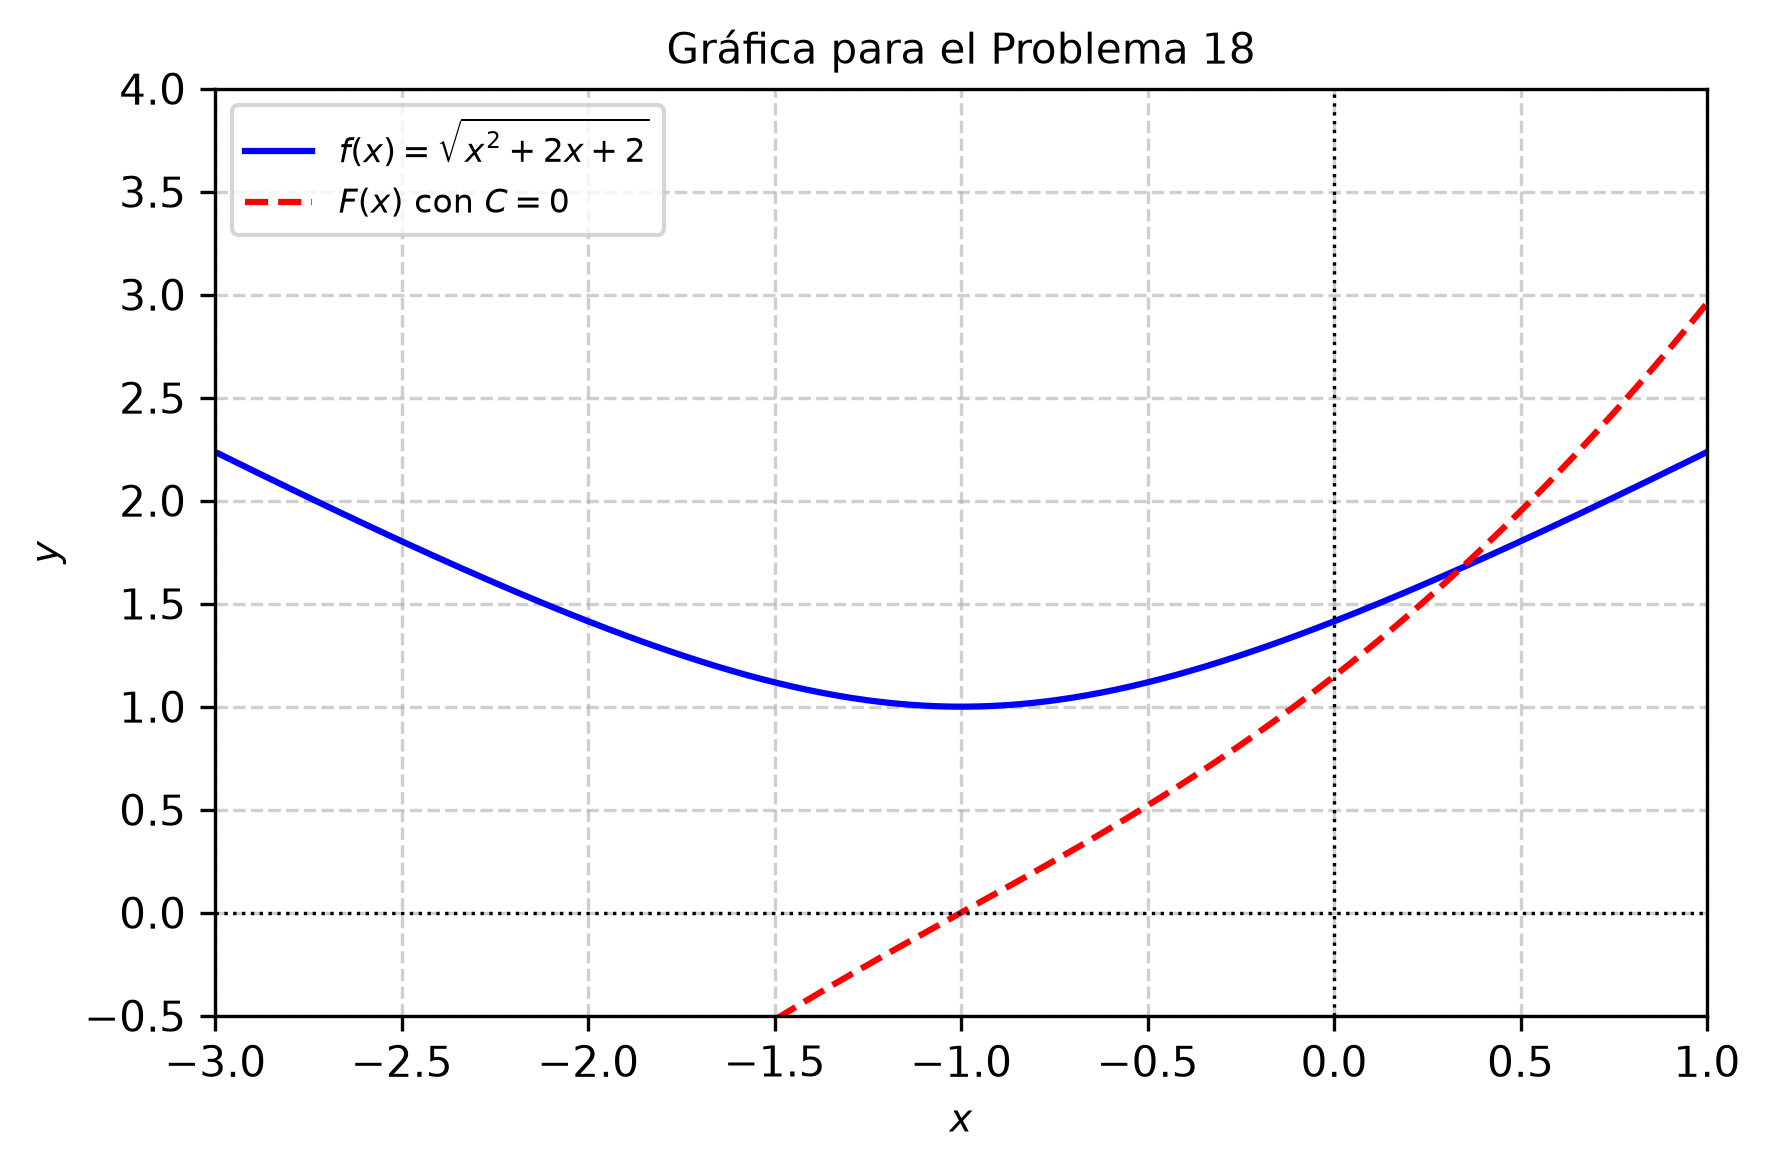
\includegraphics[width=\columnwidth]{semana_05/graficas/SEM05_P18_grafica.png}
	\caption{Representación gráfica de $f(x)$ y su antiderivada $F(x)$ evaluada para la constante de integración $C = 0$ (Problema 18).}
	\label{fig:problema18}
\end{figure}
